\documentclass[twoside,symmetric,sfsidenotes,notoc]{tufte-book}

\hypersetup{colorlinks}% uncomment this line if you prefer colored hyperlinks (e.g., for onscreen viewing)

%%
% Book metadata
\title{The HPC4Health Network}
\subtitle{Building a Canada-wide platform for human health data}
\author{HPC4Health: High-Performance Data and Computing for Health Care}
\publisher{HPC4Health}

%%
% If they're installed, use Bergamo and Chantilly from www.fontsite.com.
% They're clones of Bembo and Gill Sans, respectively.
%\IfFileExists{bergamo.sty}{\usepackage[osf]{bergamo}}{}% Bembo
%\IfFileExists{chantill.sty}{\usepackage{chantill}}{}% Gill Sans

%\usepackage{microtype}

%%
% Just some sample text
\usepackage{lipsum}

%%
% For nicely typeset tabular material
\usepackage{booktabs}

%%
% For graphics / images
\usepackage{graphicx}
\setkeys{Gin}{width=\linewidth,totalheight=\textheight,keepaspectratio}
\graphicspath{{graphics/}}

% The fancyvrb package lets us customize the formatting of verbatim
% environments.  We use a slightly smaller font.
\usepackage{fancyvrb}
\fvset{fontsize=\normalsize}

%%
% Prints argument within hanging parentheses (i.e., parentheses that take
% up no horizontal space).  Useful in tabular environments.
\newcommand{\hangp}[1]{\makebox[0pt][r]{(}#1\makebox[0pt][l]{)}}

%%
% Prints an asterisk that takes up no horizontal space.
% Useful in tabular environments.
\newcommand{\hangstar}{\makebox[0pt][l]{*}}

%%
% Prints a trailing space in a smart way.
\usepackage{xspace}

% Prints the month name (e.g., January) and the year (e.g., 2008)
\newcommand{\monthyear}{%
  \ifcase\month\or January\or February\or March\or April\or May\or June\or
  July\or August\or September\or October\or November\or
  December\fi\space\number\year
}

% Inserts a blank page
\newcommand{\blankpage}{\newpage\hbox{}\thispagestyle{empty}\newpage}

\usepackage{units}

% Typesets the font size, leading, and measure in the form of 10/12x26 pc.
\newcommand{\measure}[3]{#1/#2$\times$\unit[#3]{pc}}

% Macros for typesetting the documentation
\newcommand{\hlred}[1]{\textcolor{Maroon}{#1}}% prints in red
\newcommand{\hangleft}[1]{\makebox[0pt][r]{#1}}
\newcommand{\hairsp}{\hspace{1pt}}% hair space
\newcommand{\hquad}{\hskip0.5em\relax}% half quad space
\newcommand{\TODO}{\textcolor{red}{\bf TODO!}\xspace}
\newcommand{\ie}{\textit{i.\hairsp{}e.}\xspace}
\newcommand{\eg}{\textit{e.\hairsp{}g.}\xspace}
\newcommand{\na}{\quad--}% used in tables for N/A cells
\newcommand{\tuftebs}{\symbol{'134}}% a backslash in tt type in OT1/T1
\newcommand{\doccmdnoindex}[2][]{\texttt{\tuftebs#2}}% command name -- adds backslash automatically (and doesn't add cmd to the index)
\newcommand{\doccmddef}[2][]{%
  \hlred{\texttt{\tuftebs#2}}\label{cmd:#2}%
  \ifthenelse{\isempty{#1}}%
    {% add the command to the index
      \index{#2 command@\protect\hangleft{\texttt{\tuftebs}}\texttt{#2}}% command name
    }%
    {% add the command and package to the index
      \index{#2 command@\protect\hangleft{\texttt{\tuftebs}}\texttt{#2} (\texttt{#1} package)}% command name
      \index{#1 package@\texttt{#1} package}\index{packages!#1@\texttt{#1}}% package name
    }%
}% command name -- adds backslash automatically
\newcommand{\doccmd}[2][]{%
  \texttt{\tuftebs#2}%
  \ifthenelse{\isempty{#1}}%
    {% add the command to the index
      \index{#2 command@\protect\hangleft{\texttt{\tuftebs}}\texttt{#2}}% command name
    }%
    {% add the command and package to the index
      \index{#2 command@\protect\hangleft{\texttt{\tuftebs}}\texttt{#2} (\texttt{#1} package)}% command name
      \index{#1 package@\texttt{#1} package}\index{packages!#1@\texttt{#1}}% package name
    }%
}% command name -- adds backslash automatically
\newcommand{\docopt}[1]{\ensuremath{\langle}\textrm{\textit{#1}}\ensuremath{\rangle}}% optional command argument
\newcommand{\docarg}[1]{\textrm{\textit{#1}}}% (required) command argument
\newenvironment{docspec}{\begin{quotation}\ttfamily\parskip0pt\parindent0pt\ignorespaces}{\end{quotation}}% command specification environment
\newcommand{\docenv}[1]{\texttt{#1}\index{#1 environment@\texttt{#1} environment}\index{environments!#1@\texttt{#1}}}% environment name
\newcommand{\docenvdef}[1]{\hlred{\texttt{#1}}\label{env:#1}\index{#1 environment@\texttt{#1} environment}\index{environments!#1@\texttt{#1}}}% environment name
\newcommand{\docpkg}[1]{\texttt{#1}\index{#1 package@\texttt{#1} package}\index{packages!#1@\texttt{#1}}}% package name
\newcommand{\doccls}[1]{\texttt{#1}}% document class name
\newcommand{\docclsopt}[1]{\texttt{#1}\index{#1 class option@\texttt{#1} class option}\index{class options!#1@\texttt{#1}}}% document class option name
\newcommand{\docclsoptdef}[1]{\hlred{\texttt{#1}}\label{clsopt:#1}\index{#1 class option@\texttt{#1} class option}\index{class options!#1@\texttt{#1}}}% document class option name defined
\newcommand{\docmsg}[2]{\bigskip\begin{fullwidth}\noindent\ttfamily#1\end{fullwidth}\medskip\par\noindent#2}
\newcommand{\docfilehook}[2]{\texttt{#1}\index{file hooks!#2}\index{#1@\texttt{#1}}}
\newcommand{\doccounter}[1]{\texttt{#1}\index{#1 counter@\texttt{#1} counter}}

% Generates the index
\usepackage{makeidx}
\makeindex

\begin{document}

% Front matter
\frontmatter

% r.3 full title page
\maketitle


% v.4 copyright page
\newpage
\begin{fullwidth}
~\vfill
\thispagestyle{empty}
\setlength{\parindent}{0pt}
\setlength{\parskip}{\baselineskip}
Copyright \copyright\ \monthyear
\par\smallcaps{Published by \thanklesspublisher}
\par\smallcaps{www.HPC4Health.ca}
\end{fullwidth}

% r.9 introduction
\cleardoublepage
\chapter*{Executive Summary}

\begin{fullwidth}
The explosion of human health data can mean new advances in human health care ---
but only if the infrastructure, architecture, policies, and expertise are brought
together in innovative ways to make effective, safe research use of the data.
We have such an example of a collaborative center in Canada, in HPC4Health.

An innovative and successful shared platform for health genomics data and analysis,
the original incarnation of HPC4Health in 2014 was a small pilot project between
SickKids and UHN; today, the collaboration counts amongst its employees six scientific 
and eight technical staff, works with four partner institutions, and provides 7,000
compute cores and over 2 petabytes of secure data storage.

With continued success both technical and scientific HPC4Health faces a question --- 
how best to expand to meet growing demand in institutions across Canada.  Should 
the organization meet growing by increasing the capacity of its current operations,
or by developing more such operations across the province, and connecting them
all into a coherent whole?

While current facilities have room to grow, there are several factors that will limit
scaling HPC4Health as a centralized resource over time.  As with any data-intensive science,
the need to keep compute near the modern high-throughput data generation facilties,
and the desire to make use of local clusters of expertise and resources, both suggest
against single, centralized facilities.  And in the particular case of human health, 
data governance policies may require a more decentralized approach.

The H4H Network, with pilot projects already in place in Montr\'eal and
Hamilton, will build a coherent, shared network of resources and expertise available
to health researchers across Canada.  With each site modelled after the current HPC4Health
site at SickKids, the network will use: a single, coherent security policy; a common
software stack; and a federated network of genomic experts, all presenting a common
set of services to researchers while providing international best-practices in security, privacy,
and governance.  The H4H Network will unlock genomic data and local expertise for
benefit of all Canadians, while maintaining the security and privacy of all
patient data.
\end{fullwidth}

%%
% Start the main matter (normal chapters)
\mainmatter

\chapter{Human Health Research in the Era of Genomics}
\label{ch:health-data-at-scale}

\newthought{Next-generation genomics and electronic medical records} have 
become ubiquitous almost simultaneously, opening completely new windows onto the field
of human health research.  

\begin{figure}
 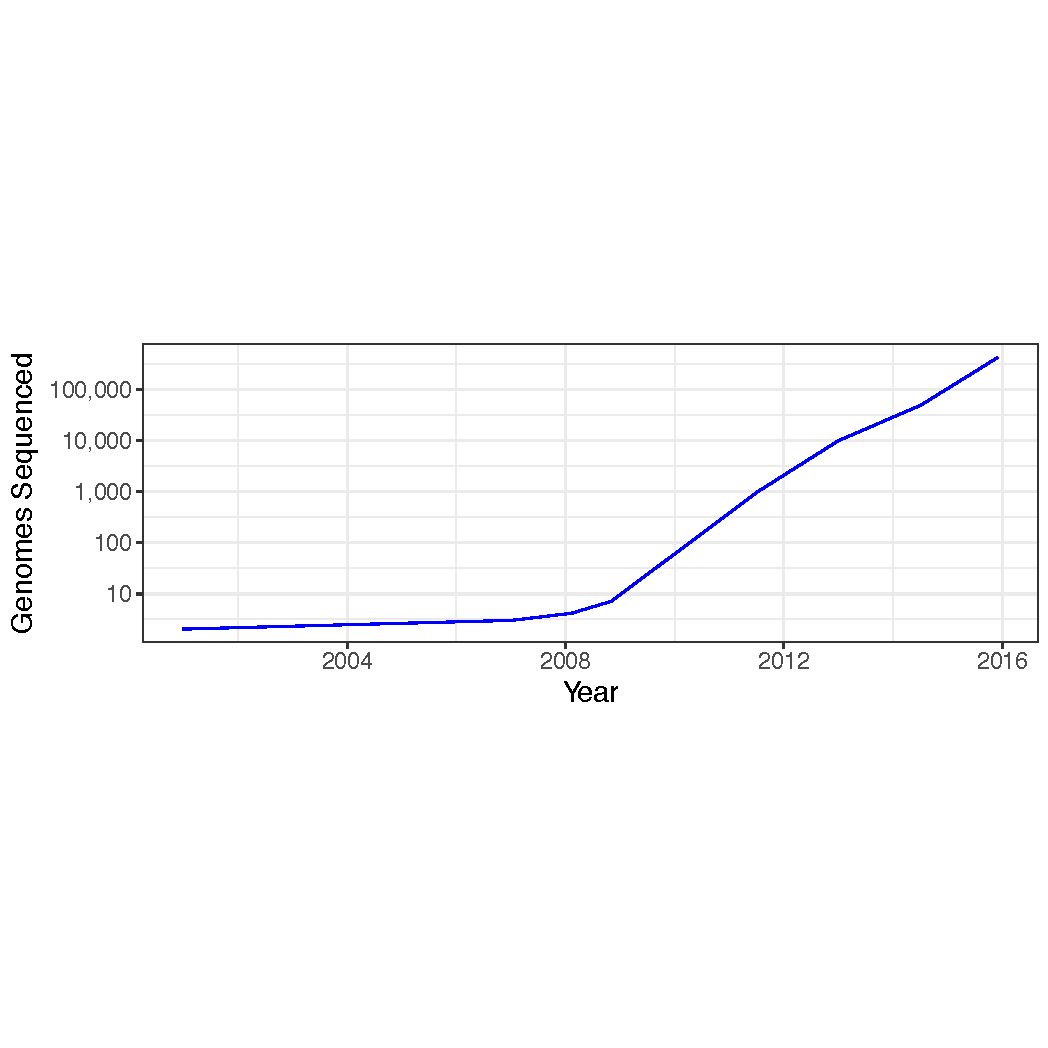
\includegraphics{cumulative_genomes.pdf}
  \caption[Cumulative number of human genomes sequenced]{The cumulative number of human genomes sequenced over the past 15 years,
    data from \protect\citep{stephens2015big}.  New technologies and data types have caused a inflection in the exponential rate
    of data growth which continues today.}
  \label{fig:exponential-growth}
\end{figure}

In genomics\footnote{\textit{Genetics} is the study of single genes
and their role in the heredity of conditions. \textit{Genomics}
describes the study of an individual's genome -- the totality of
all of their genetic information.}, an exponentially-growing number of human genomes are
being sequenced, creating enormous amounts of evidence on the heredity
of human disease states at previously inaccessible levels of detail
(Fig~\ref{fig:exponential-growth}).  Data rates are only increasing as
new devices become available, and new types of data are being
generated; for instance, RNA sequencing allows us to go beyond
simply sequencing ``the'' genome of an individual and instead measure
the gene products being expressed in particular cells at particular
times, giving us insight into not just predispositions but the precise
disease state of cells over time.

Until now, the bulk of this genomic data has come from research projects ---
focused, generally short-term efforts to answer specific questions using 
genomic information. However, two changes in the practice of medicine are
poised to radically increase the rate of genomic and human health data creation
in Canada.

First, genomic medicine\footnote{\textit{Genomic Medicine} is a term used by NIH's
National Human Genome Research Institute and others to describe medicine 
that uses genomic information about an individual 
for diagnostic or therapeutic decision-making.} is beginning
to enter the standard of care, initially in the cases of hard-to-diagnose
rare diseases or recurrent cancers, and starting to displace smaller
and more limited genetic tests in other areas.  The sheer scale of clinical medicine 
--- in Canada, hospital spending alone is nearly seventy times the research funding
budget of the CIHR --- means that as adoption increases, clinical
genomic data creation will rapidly and decisively outpace that of research genomic data.

Second, information technology advances elsewhere in healthcare
has led to the rapid adoption of Electronic Medical Record systems\footnote{
\textit{Electronic Medical Records}, or EMRs, are digital version of paper chapters
in hospitals or doctors offices; \textit{Electronic Health Records}, or EHRs, are
more integrated systems combining information across practices and institutions.
EMRs are mature and growing in adoption rapidly, while EHR systems are still
some time from being common.}, describing a patient's condition, tests, and
treatment in detail and at least partially in machine-readable form.

The rapid growth of genomic data volumes and the increasing depth and detail
of clinical data present in EMRs offers enormous promise for human health research,
with insights into both basic biology and to future treatments.  The joint analyses
of clinical and phenotypic health record data along with genomic information 
about the patient and their disease offers unprecented opportunity for researchers
to connect genetic predisposition, treatments, and outcomes, allowing the
development of national, truly precision, medicine practices.

But making use of this data in an era of rapid growth raises multiple challenges.
On the physical infrastructure side, simply making available the storage 
resources to capture and archive the onrush of data is a daunting effort, along with
providing the computational power to perform increasingly sophisticated analyses.
Architecting, building, and maintaining these systems, particularly tuned to
the needs of health research, requires a specialized approach.

Human infrastructure is also required.  Making productive use of the 
data means ensuring that the expertise exists and is available to for interpretation,
that those experts are continuously kept up to date on the new types of data
and new techniques for analysis, and have time to develop novel methods to address
the questions they are tasked with answering.  This requires funding, ongoing training,
and opportunities for professional recognition and growth of the experts, whether
they be bioinformaticians, computational biologists, or systems administrators.

Finally, the unique challenges of dealing with health data means that the duty
of care to patients to zealously protect the security and their privacy is
paramount; sophisticated and enforcable policies around data governance and consent
are required, along with international best practices around security and monitoring.

The explosion of human health data can mean new advances in human health care ---
but only if the infrastructure, architecture, policies, and expertise are brought
together in innovative ways to make effective, safe research use of the data.
We have an example of such a collaborative center in Canada, in HPC4Health.

\chapter{HPC4Health --- a Made-in-Canada Approach}
\label{ch:hpc4health}

\newthought{As early and major players in genomic research and medicine}, in 2014 SickKids and 
the University Health Network (UHN) faced a problem --- how to manage and make use of the influx 
of genomic and other health data they were already charged with storing and analyzing.

With a common challenge, and building on existing partnerships, the institutions formed a
first-of-its-kind collaboration and in Canada, combining forces and sharing
resources to build HPC4Health\footnote{\url{http://www.hpc4health.ca}}: a
shared-services approach, building a cross-institution center
of infrastructure and expertise
for the computational analysis of human health and genomic data.  This innovative 
partnership gathered much attention in the hospital, genomics, and 
research computing communities \citep{hn-hpc4health, gw-hpc4health, inside-hpc-h4h-mellanox, openstack-hpc}.

\begin{figure}
  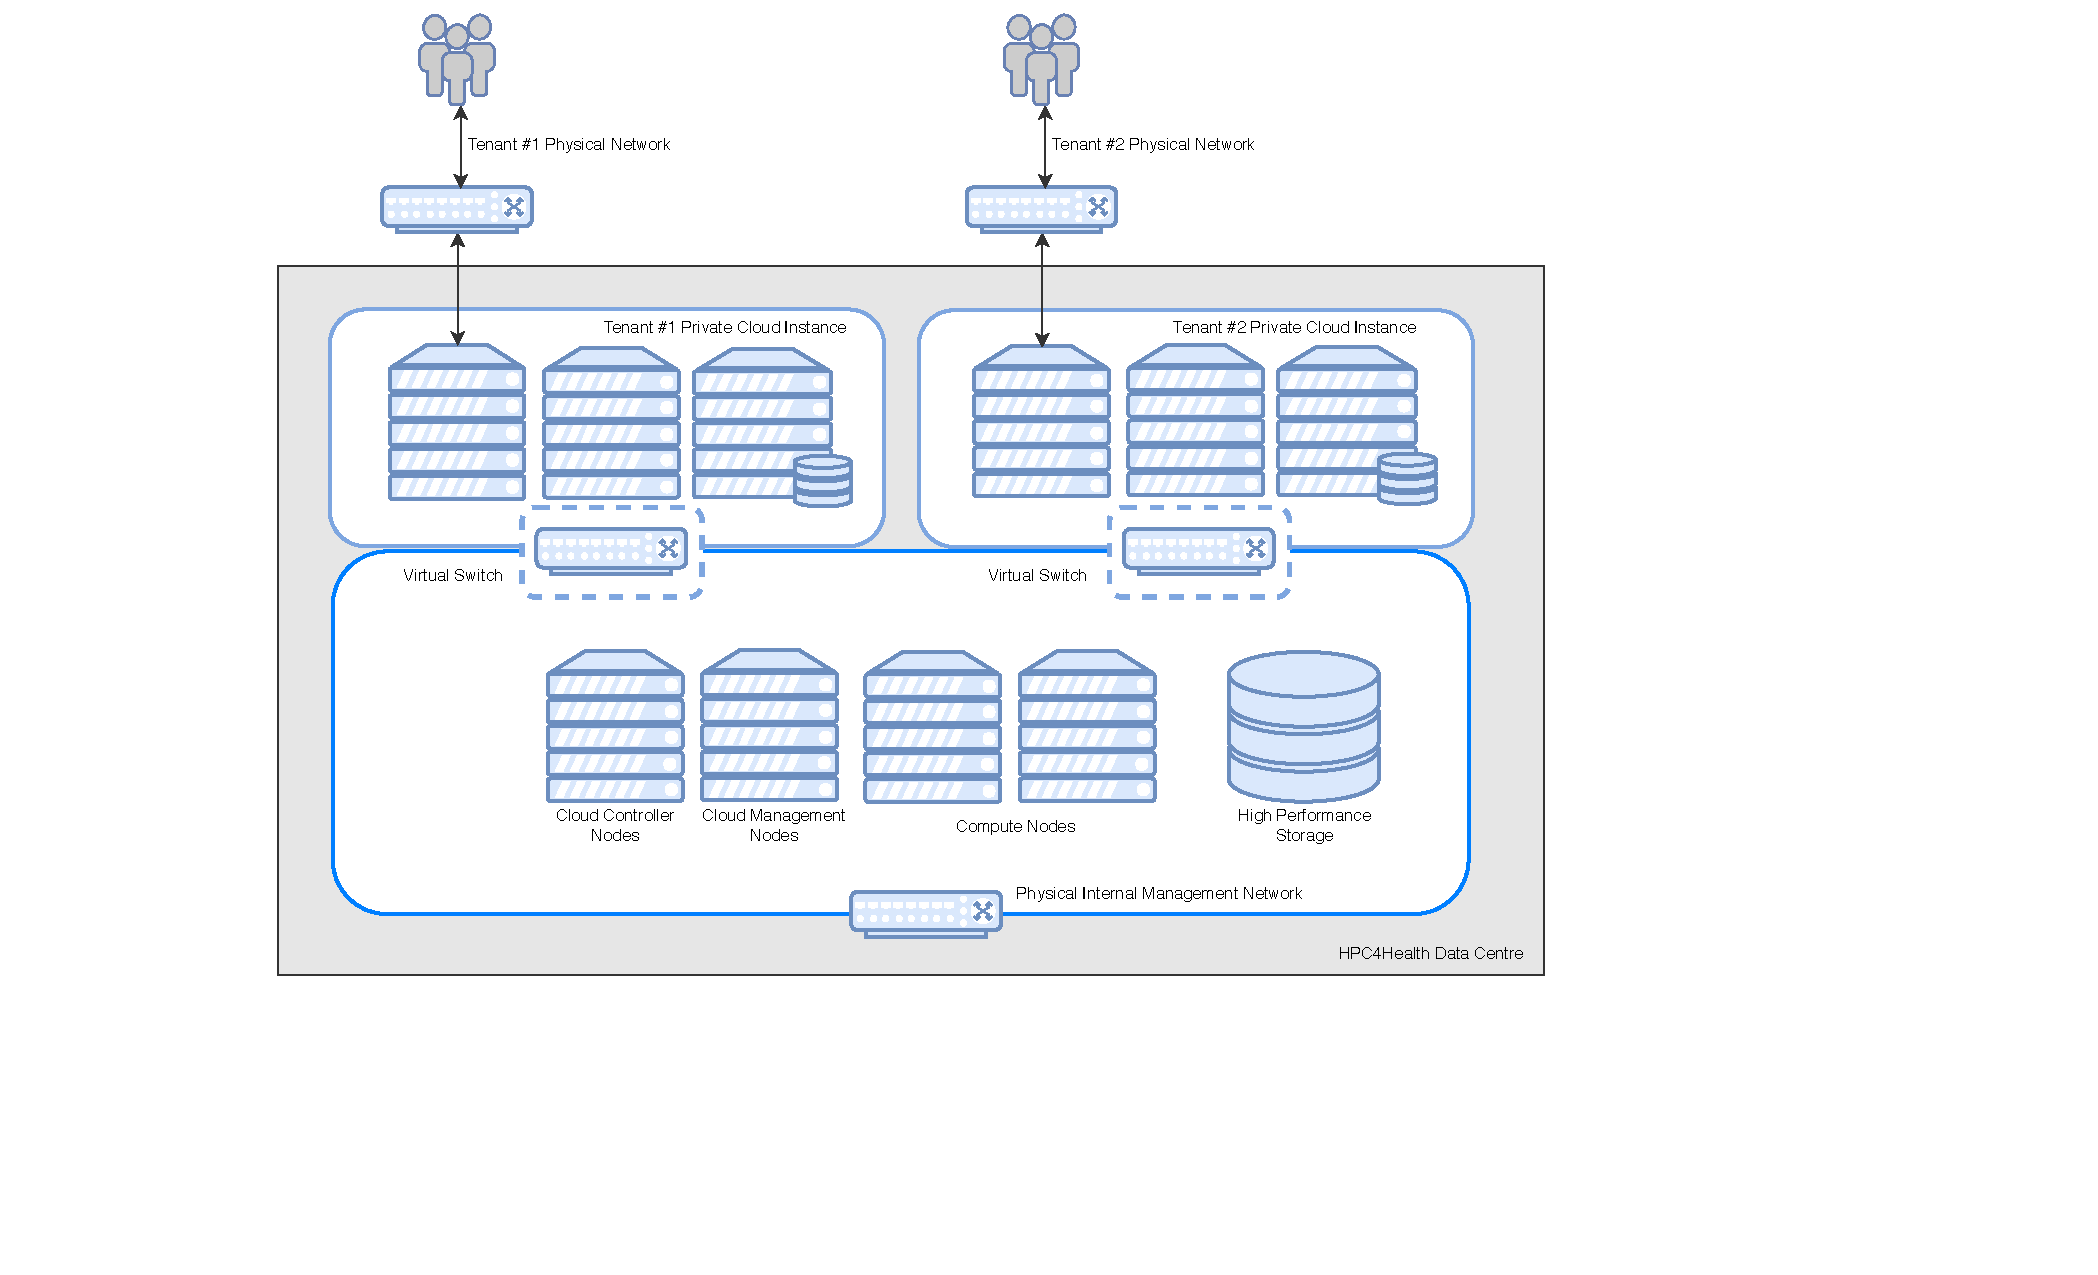
\includegraphics{HPC4Health_1.pdf}
  \caption[HPC4Health Architecture Diagram]{The HPC4Health Architecture.  An on-premesis (at SickKids) private
  cloud is partitioned into tenant-controlled secure data environments for the institutions, with shared administrative
  resources managed by the HPC4Health administrators.  Tenants can get technical support from the core
  technical staff, or scientific support from the growing team of genomics, machine learning, and
  medical record experts. }
  \label{fig:hpc4health-architecture}
\end{figure}

HPC4Health's compute and storage infrastructure (Fig~\ref{fig:hpc4health-architecture})
consists of an elastic secure cloud --- an arrangement that functions like an commercial building
rented to multiple tenants.  The ``superintendant'' maintains core shared facilities, but
the ``tenants'' have complete control of their own office space.   This is implemented through
in an on-premises private OpenStack\footnote{\url{https://www.openstack.org}} cloud,
partitioned securely into an administrative core and ``tenant'' environments.

Crucially, HPC4Health is more than computational infrastructure;  it is also
experience and expertise.  HPC4Health is governed by a sophisticated
policy and data governance framework; it is managed and advised by an executive committee
and a science advisory panel; and is run by teams of technical and scientific
personnel that every day make sure that health insight is successfully distilled from
health data.

The original incarnation of HPC4Health in 2014 was a small pilot project between
SickKids and UHN; today, the collaboration counts amongst its employees six scientific 
and eight technical staff, works with four partner institutions, and provides 7,000
compute cores and over 2 petabytes\footnote{A \textit{petabyte} is over a million gigabytes,
and is enough to store over three years worth of 24/7 high-definition video, or 
raw data from nearly 7,500 whole genome sequencing experiments.} of secure data storage
from its primary data centre in SickKids research institute building.

With continued success both technical and scientific (with over XXX \textbf{TODO}
publications), HPC4Health faces a question --- how best to expand to meet growing demand
in institutions across Canada.  Broadly, should HPC4Health meet demand by scaling
vertically or horizontally\footnote{Scaling a system \textit{vertically}, or ``scaling up'',
means making the components of a system more powerful --- bigger, faster,  greater capacity ---
while scaling \textit{horizontally}, or ``scaling out'', means increasing the number of
components.  The benefits of horizontal scaling when appliciable are generally flexibility,
cost-effectiveness, and fault-tolerance, while that of vertical scaling are typically 
simplicity.}; should HPC4Health serve more researchers by increasing the capacity of
its current operations, or by developing more such operations across the province, and
connecting them all into a coherent whole?

While HPC4Health operations has room to grow, there are several factors that will limit
the feasibility of vertical scaling over time; many of these are common to data-intensive
science generally:

The first concerns the importance of \textit{keeping compute near the data generation}.  Data generation rates of modern devices
are growing much more quickly than network speeds. Individual modern sequencing devices
can output data in excess of 1,000 gigabytes per hour, straining or saturating wide-area
network links.

The second involves \textit{making efficient use of local resources and expertise}.  significant investments have been
made across Canada in training of both highly qualified personnel, often in clusters with 
significant expertise in particular problems or analyses types, and in equipment.  Making
effective use of those resources is crucial to cost-effective expansion.

Finally, consistancy with existing \textit{data governance policies} is a hard requirement.
Many stewards of human health data, who legally and ethically have extremely strict 
responsibilities for the data entrusted to them by patients, have policies in place
about keeping data on-premesis or limiting where the data can go (such as going to another
jurisdiction) or who can be in control it.


\chapter{The H4H Network --- Building on Strengths}
\label{ch:hpc4health_network}

\newthought{To build on both HPC4Health successes and strengths and investments elsewhere},
we take a system-wide approach with the H4H Network --- allowing the benefits of coordation
such as economies of scale from consistent design, shared procurement, unified management;
consistent services for researchers; and best-practice security adminstration --- while also
taking advantage of local clusters of expertise and resources, and placing facilites near
data generation.

\begin{figure}
  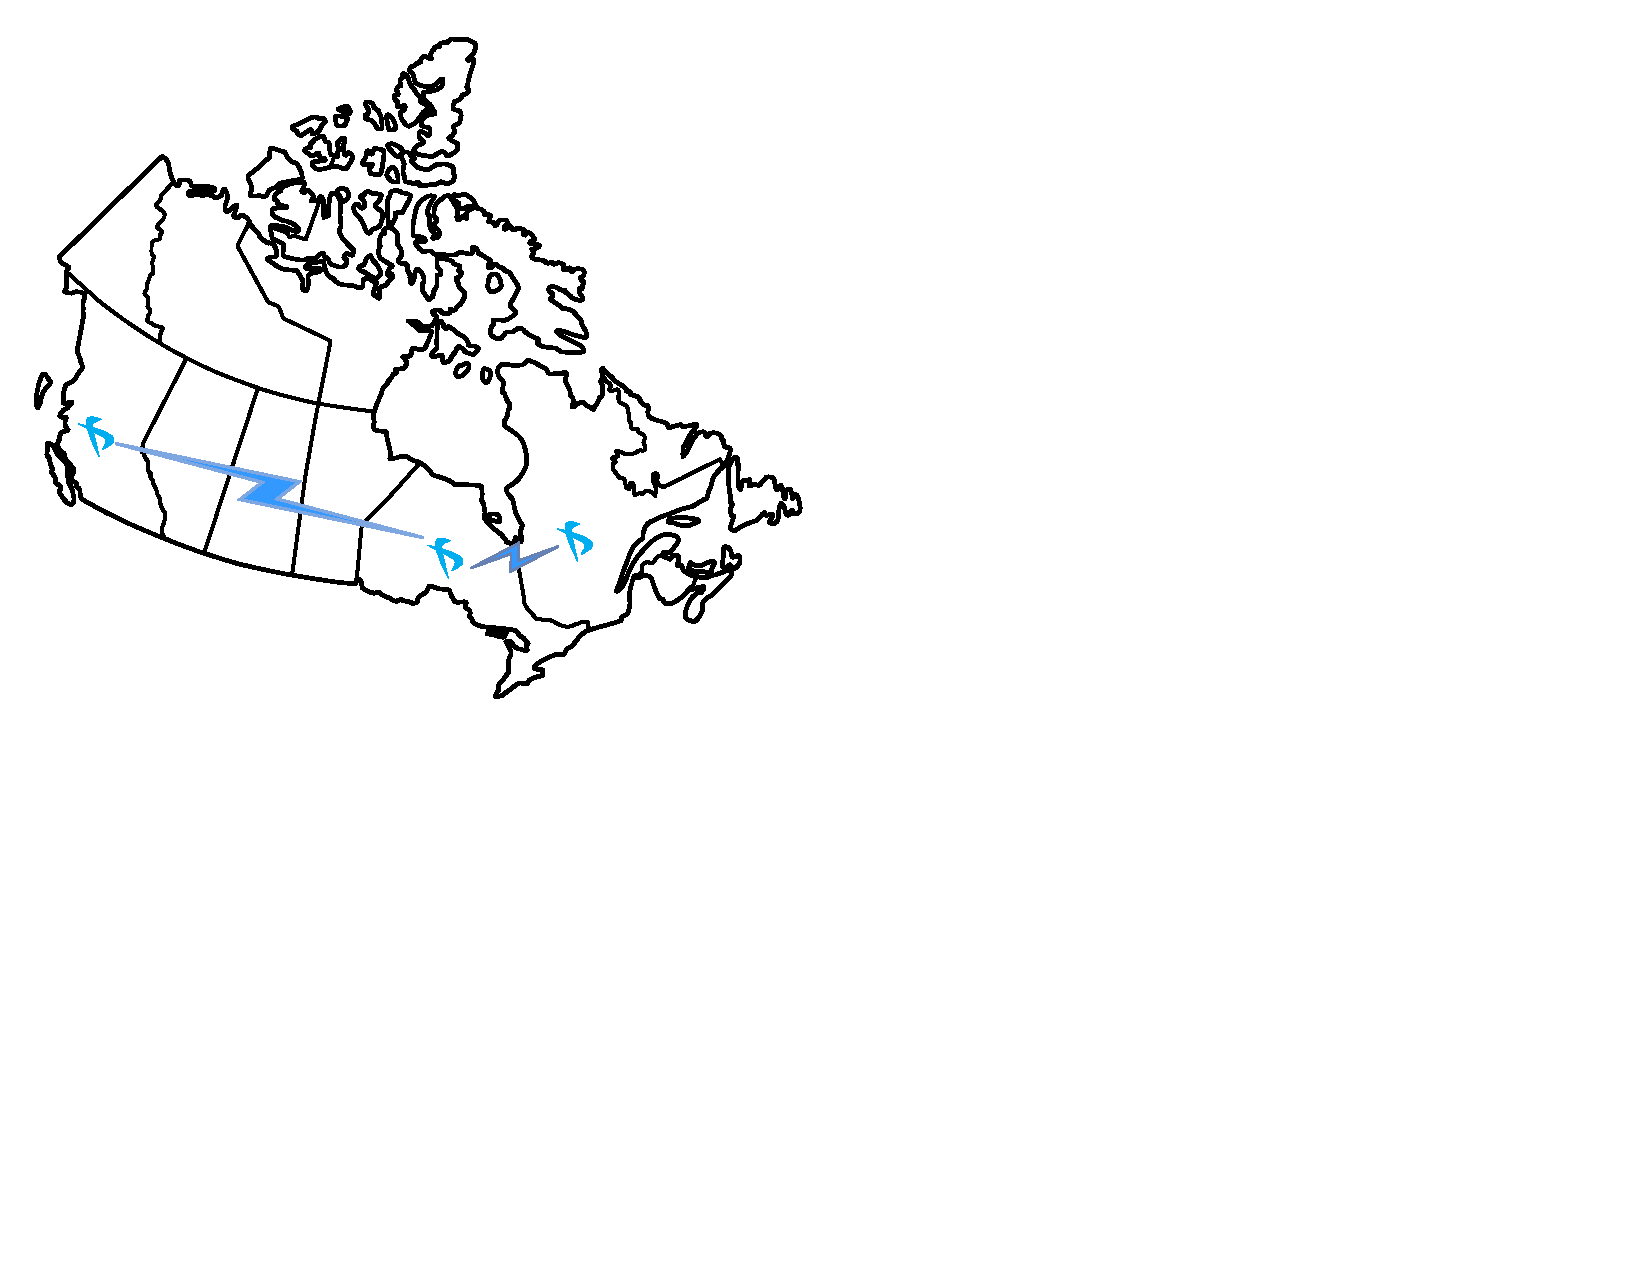
\includegraphics{H4HNetwork_Canada.pdf}
  \caption[The H4H Network]{The H4H Network, with pilot projects already in place in Montr\'eal and
  Hamilton, will build a coherent, shared network of resources and expertise available to health 
  researchers across Canada.  With each site modelled after the current HPC4Health site at SickKids,
  the network will use: a single, coherent security policy; a common software stack; and a federated
  network of genomic experts, all presenting a consistent services to researchers while providing 
  international best-practices in security, privacy, and governance.}
  \label{fig:hpc4health_network}
\end{figure}

Pilot projects implementing secure health cloud systems modelled after HPC4Health at both McMaster
and McGill have demonstrated the feasibility and
utility of exporting the HPC4Health architecture.  But for researchers to make the best
possible use of the health data entrusted to them by patients, and to take advantage of scale
in purchasing, administration, and security, it is not enough to have Canada's genomic research
data isolated in identical silos.  These sites must be part of a connected network, with researchers able
to access the combined expertise --- and, when appropriately authorized, particticular 
data sets --- from across the network.

The next step for the H4H Network is, starting with existing pilots, to build 
that secure network of human health data sites, with coherent policies, security 
domain and monitoring, and with data available for analysis by researchers using
existing projects and services such as GenAP\footnote{\href{https://genap.ca}{genap.ca}}
and CanDIG\footnote{\href{https://www.distributedgenomics.ca}{distributedgenomics.ca}}.

We propose to begin by expanding the Hamilton site and unifying it with common
security domain, operational procedures, and data governance policies; and once those
policies have been successfully developed to encompass multiple sites, expanding 
to a fourth site at one of several possible institutes.

%%
% The back matter contains appendices, bibliographies, indices, glossaries, etc.

\backmatter

\bibliography{h4h_network}
\bibliographystyle{plainnat}


\printindex

\end{document}